% !TeX spellcheck = it_IT
%Cambio slide

\section{Wireless Personal Area Network WPAN}

\subsection{ISM Band}
Ci sono \textbf{porzioni di banda unlicensed}, ovvero che non necessitano di licenza per essere utilizzate. Sono riservate per usi industriali, scientifici e medici (ISM).\\

Bluetooth, Wi-Fi, apparecchi medici e tutti i dispositivi wireless comunicano sulle stesse frequenze. Essendo condiviso, le varie tecnologie devono tollerare interferenze.\\

\subsection{Pulse Code Modulation PCM}
Si tratta di una codifica lossless per onde. Partendo da un segnale continuo, l'ampiezza della curva viene quantizzata in livelli (intervalli) e viene effettuato un campionamento. La frequenza di campionamento è il doppio della frequenza massima da campionare (Teorema del campionamento di Shannon).

\begin{center}
	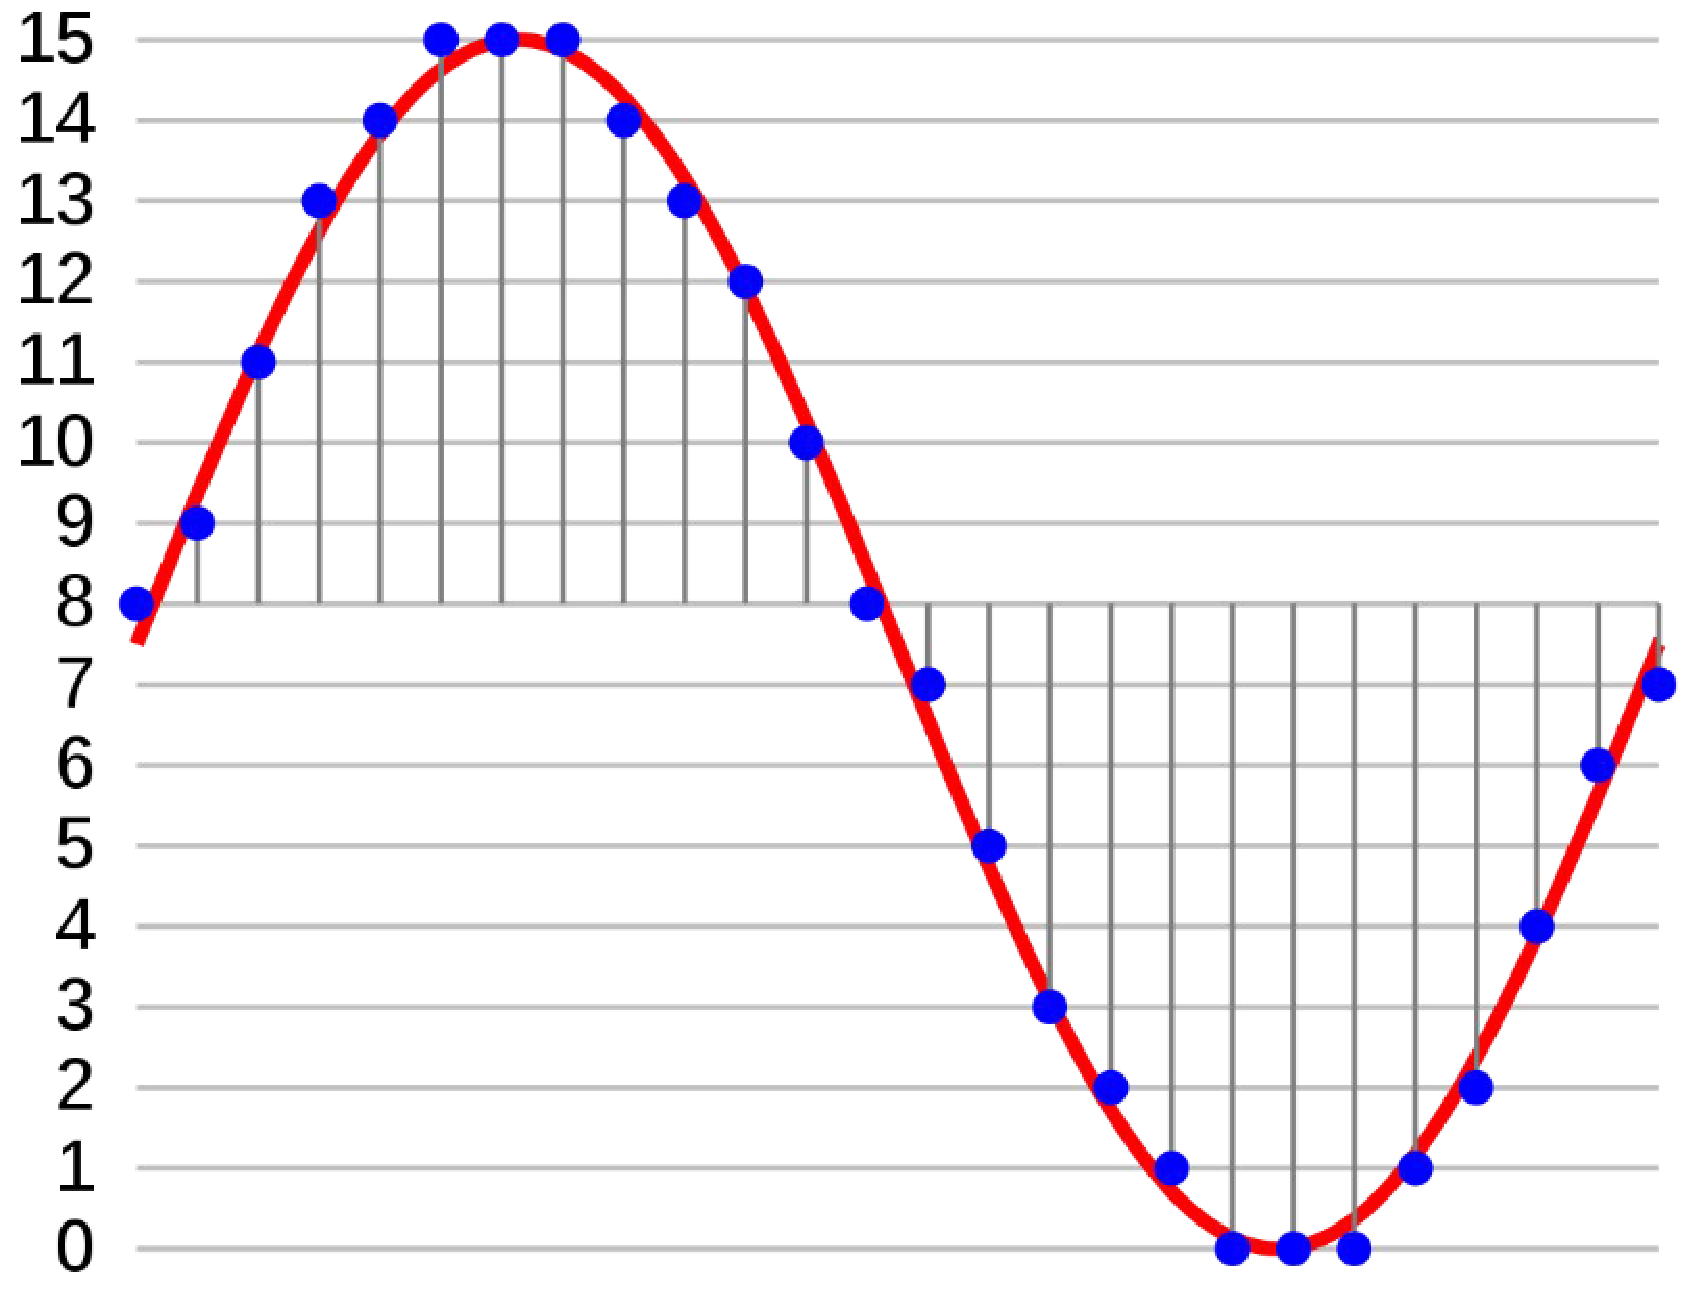
\includegraphics[width=0.7\linewidth]{img/wpan/PCM}
\end{center}

Per la voce telefonica: PCM 8bit $8000Hz$, quindi $64kbps$ (frequenza della voce $300 - 3400 Hz$). La musica viene campionata a 24bit $41/48kHz$.\\

\subsection{802.15.x}
Lo standard 802.15 comprende un insieme di tecnologie per la \textbf{comunicazione a corto raggio} (\texttt{\url{https://www.ieee802.org/15/}}).\\

Esempi di tecnologie: 
\begin{itemize}
	\item 802.15.1 Bluetooth
	\item 802.15.2 High-rate WPAN
	\item 802.15.4 Low-rate WPAN (es. Zigbee)
	\item 802.15.5 Mesh Networking (combinazione di High-rate e Low-Rate)
	\item 802.15.6 Body Area Network (BAN) pensato ad esempio per applicazioni in ambito medico
	\item 802.15.7 Visible Light Communication (VLC) (es. Vehicle-to-vehicle communication \& Li-Fi)
\end{itemize}

\subsection{Bluetooth}
Si tratta dello standard 812.15.1. Si compone di reti chiamate piconet ed all'interno della rete si ha un dispositivo \textbf{master} e \textbf{uno o più slave} sotto il controllo del master, che controlla la piconet.\\

\textbf{Caratteristiche}: 
\begin{itemize}
	\item Short range (10-50m nei casi d'uso tipici a seconda della classe di potenza del dispositivo, \texttt{\href{https://www.bluetooth.com/learn-about-bluetooth/key-attributes/range/\#estimator}{Bluetooth range estimator}})
	\item Usa la banda ISM $2.4GHz$
	\item Data Rate: $2.1 Mbps - 24Mbps$
\end{itemize}

Utilizzi: 
\begin{itemize}
	\item punto di accesso per dati e voce
	\item sostituzione di cavi (periferiche wireless)
	\item comunicazione ad hoc con altri dispositivi Bluetooth
\end{itemize}

\newpage

\subsubsection{Architettura dei protocolli} 
\begin{center}
	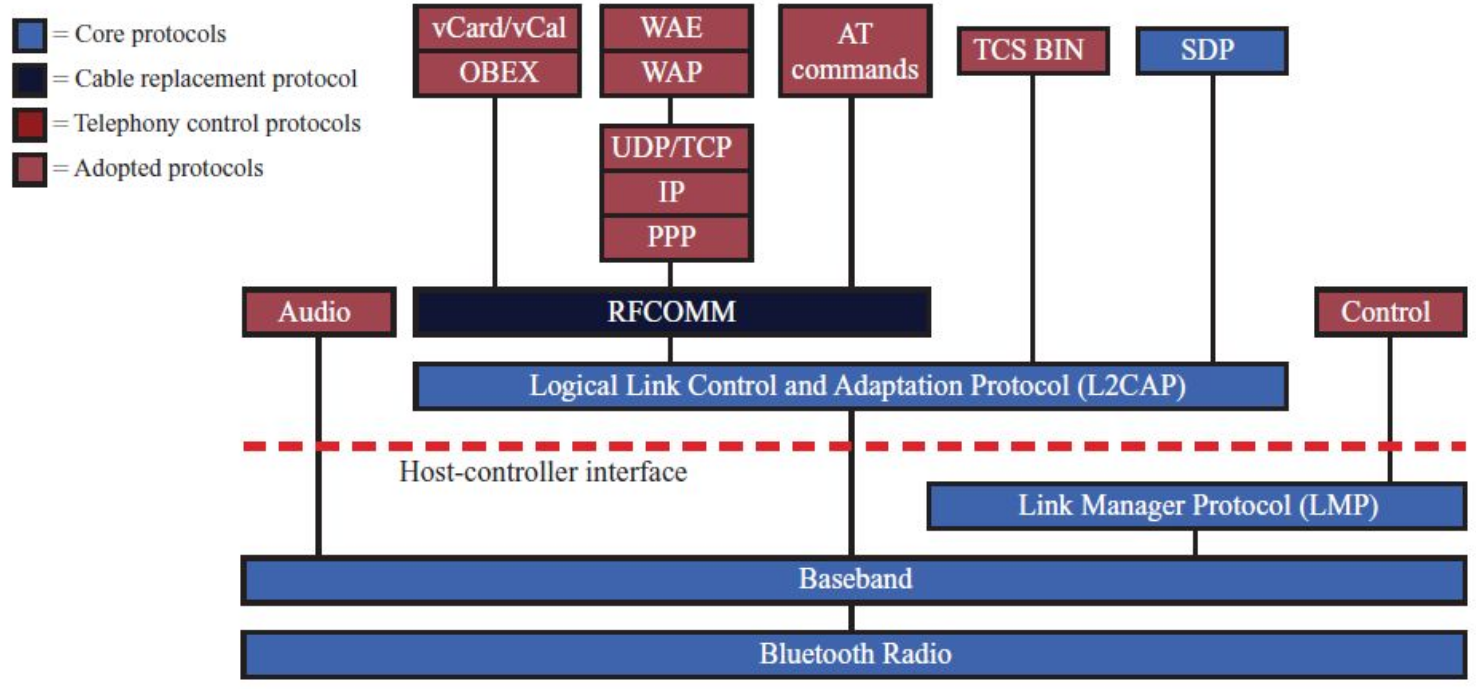
\includegraphics[width=0.95\linewidth]{img/wpan/archbt}
\end{center}
In blu sono i "core protocols", presenti in tutti i dispositivi Bluetooth. Gli altri (rossi e blu scuro) sono implementati solo se il dispositivo ne necessita, in base all'uso.\\

\paragraph{Bluetooth Radio:} La parte di livello fisico, specifica l'interfaccia radio: 
\begin{itemize}
	\item radio frequenze, quali frequenze utilizzare
	\item gestisce il frequency hopping
	\item decide lo schema di modulazioni in base al canale
	\item determina la potenza di trasmissione
\end{itemize}

\paragraph{Baseband:} Il livello di Baseband si occupa di 
\begin{itemize}
	\item stabilire la connessione con la piconet
	\item gestire l'indirizzamento
	\item formattazione dei pacchetti (frame)
	\item gestire le tempistiche di comunicazione (Time Division Duplex TDD e Time Division Multiple Access TDMA)
	\item gestisce la potenza di trasmissione (passa le indicazioni a livello radio)
\end{itemize}

\paragraph{Link Manager Protocol LMP:} Fa da "manager" del collegamento. Si occupa di:
\begin{itemize}
	\item configurare i collegamenti tra dispositivi
	\item gestione di collegamenti attivi
	\item funzionalità di sicurezza e cifratura
\end{itemize}
Si tratta di un protocollo di controllo, non passano dati ma gestisce il collegamento per i livelli sottostanti.

\paragraph{Logical Link Control and Adaptation Protocol (L2CAP):} I livelli precedenti erano implementati sul chip Bluetooth, da qui in su vengono implementati a livello software. Si occupa di:
\begin{itemize}
	\item adatta i protocolli di livello superiore al livello baseband
	\item astrarre tutto ciò che c'è sotto per i servizi a livelli superiori, \textit{Connectionless} e \textit{Connection-oriented}
\end{itemize}

\paragraph{Service Discovery Protocol SDP:} Gestisce le informazioni del dispositivo. Permette di comunicare
\begin{itemize}
	\item servizi disponibili sul dispositivo
	\item caratteristiche sul dispositivi
\end{itemize}
Stile architettura client-server: prevede interrogazioni richiesta-risposta per stabilire connessioni tra dispositivi Bluetooth.

\paragraph{Radio Frequency Communication RFCOMM:} Astrae il livello di Bluetooth, permette di "astrarre un cavo". Simula una comunicazione seriale e permette la trasmissione di dati tra dispositivi Bluetooth.

\paragraph{Livelli superiori:} I livelli in rosso sono protocolli "già esistenti", ciascun dispositivo può avere parte di questi protocolli in base all'uso, i livelli inferiori permettono la comunicazione a livello fisico.\\

\newpage

\paragraph{Profili:} Per avere determinate funzionalità un dispositivo deve seguire dei "profili". Esempi di profili:
\begin{center}
	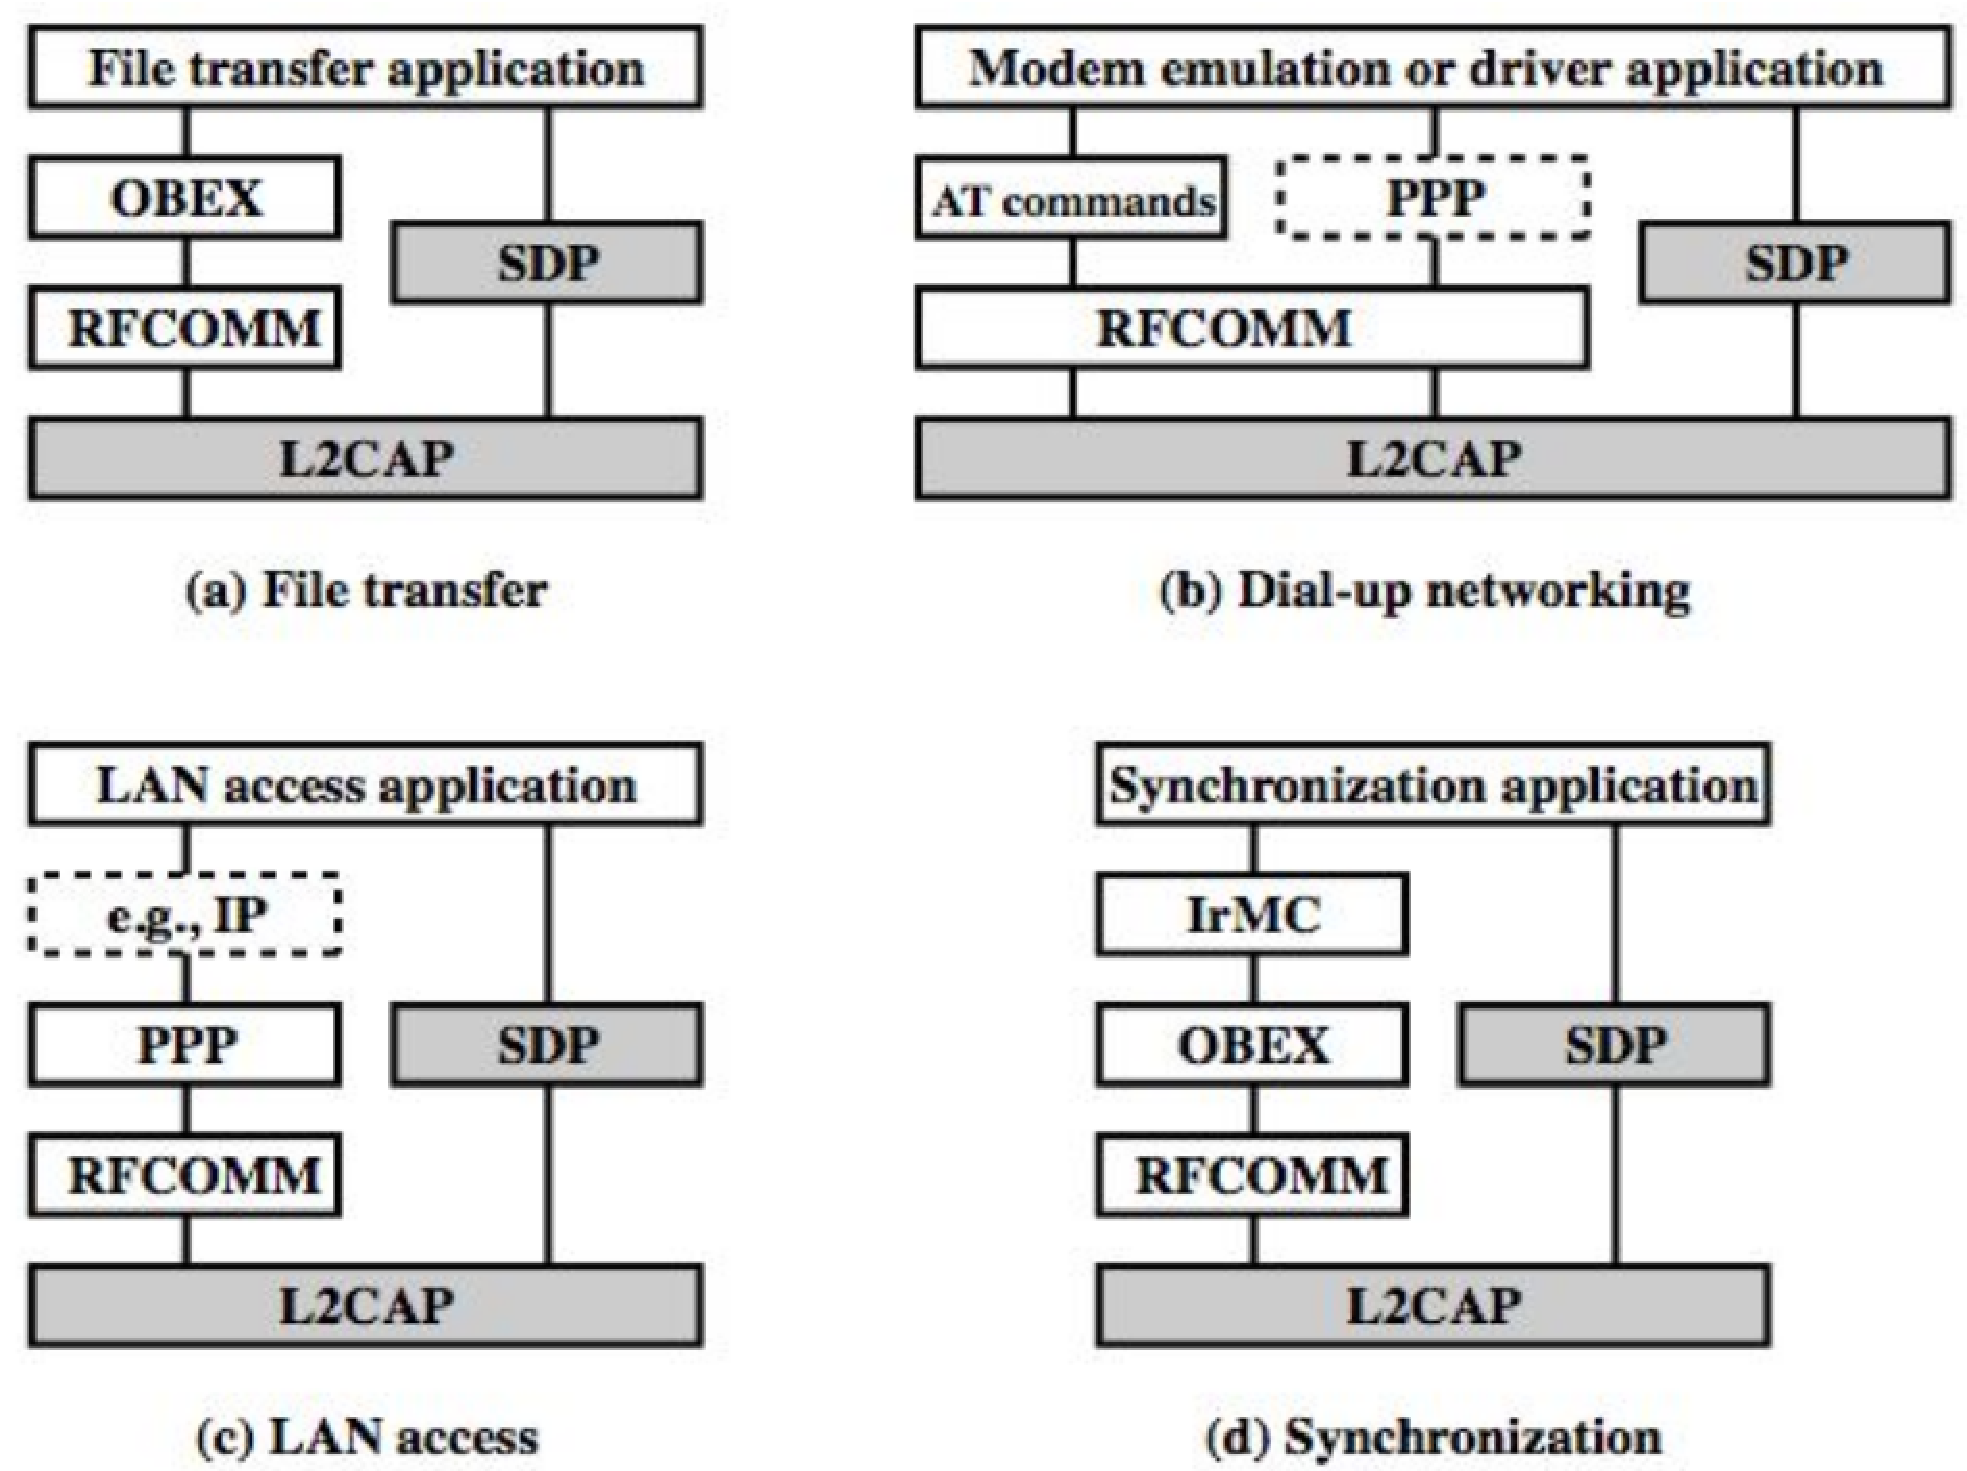
\includegraphics[width=0.7\linewidth]{img/wpan/profiles}
\end{center}
Questi sono standard, un dispositivo deve aderire ad uno o più profili (annunciati dal SDP) per avere il relativo utilizzo.\\

\newpage

\subsubsection{Piconet \& Scatternet}

\paragraph{Piconet:} Una piconet è composta da un \textbf{master} e 
\begin{itemize}
	\item \textbf{Active Slave (AS)}: membro attivo delle piconet, con un indirizzo Active Member Address (AMA) su 3 bit assegnato dal master (0 è il master, quindi 7 dispositivi al massimo)
	\item \textbf{Parked Slave (PS)}: membro della piconet ma temporaneamente disattivato, non possono comunicare attivamente ma solo ogni tanto tramite il Parked Member Address (PMA), 8 bit (0 è il master); un parked può tornare attivo solo se "c'è spazio"
	\item \textbf{Standby Slave (SS)}: non sconosciuti ma scollegati; non hanno indirizzi e possono quindi essere infiniti
\end{itemize}
\begin{center}
	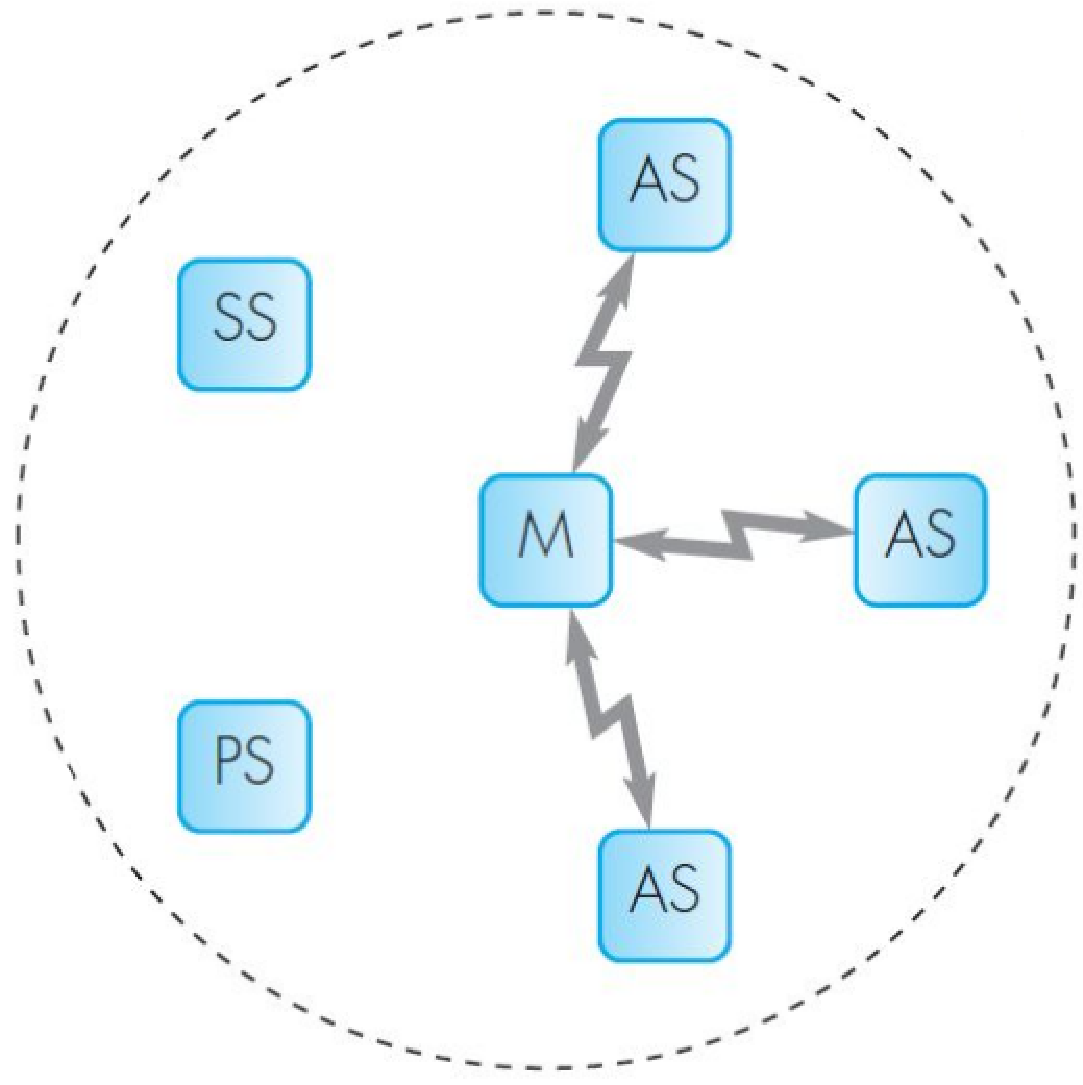
\includegraphics[width=0.35\linewidth]{img/wpan/pico1}
\end{center}

\paragraph{Scatternet:} La piconet ha al centro sempre un master, ma un dispositivo può appartenere a più piconet, portando ad una scatternet
\begin{center}
	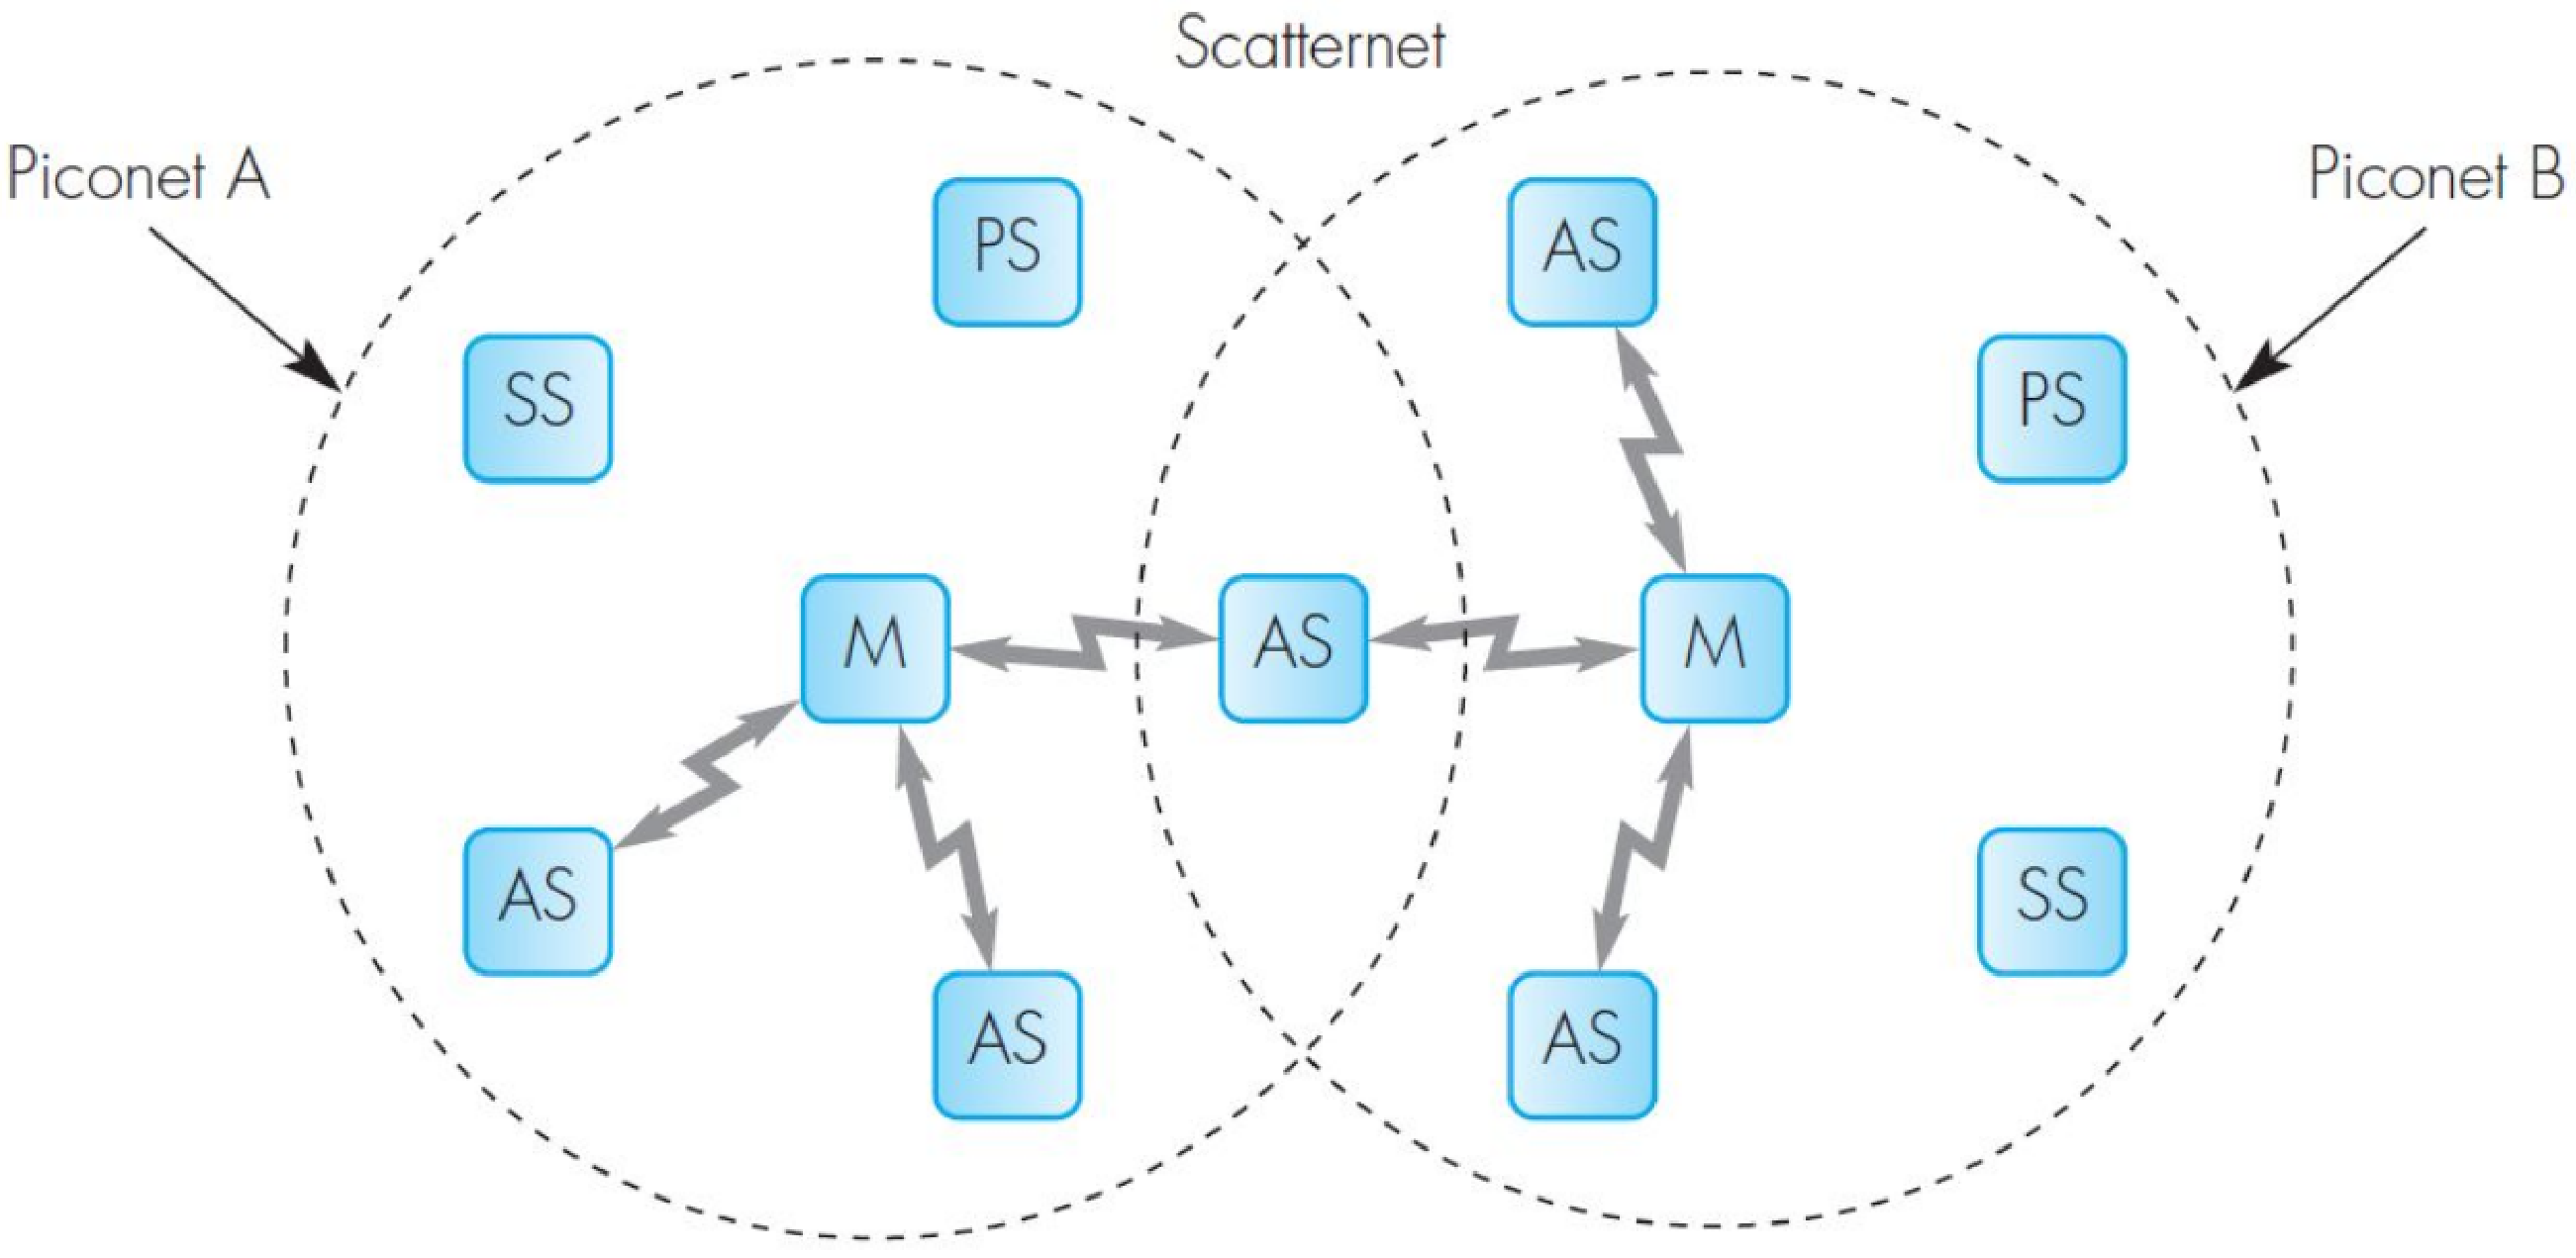
\includegraphics[width=0.7\linewidth]{img/wpan/scatter}
\end{center}
In qualsiasi caso i master lavorano in maniera completamente \textbf{separata}. Un AS attivo in due piconet diverse avrà indirizzamento diverso sulle due reti.

\subsubsection{Specifiche Bluetooth}
\paragraph{Specifiche radio Bluetooth 2.1:}
\begin{center}
	{
	\resizebox{0.98\textwidth}{!}{
	\renewcommand{\arraystretch}{1.2}
	\begin{tabular}{|l|l|l|}
		\hline
		& \textbf{Basic Rate (BR)} & \textbf{Enhanced Data Rate (EDR)} \\ 
		\hline
		\textbf{Topology} & \multicolumn{2}{c|}{Up to 7 simultaneous links in a logical star} \\ 
		\hline
		\textbf{Modulation} & GFSK & $\pi/4$-DQPSK and 8DPSK \\ 
		\hline
		\textbf{Peak data rate} & $1 Mbps$ & $2 Mbps$ and $3 Mbps$ \\ 
		\hline
		\textbf{RF bandwidth} & \multicolumn{2}{c|}{$220 kHz (-3 dB)$, $1 MHz (-20 dB)$} \\ 
		\hline
		\textbf{RF band} & \multicolumn{2}{c|}{$2.4 GHz$, ISM band} \\ 
		\hline
		\textbf{RF carriers} &  \multicolumn{2}{c|}{$23/79$}  \\ 
		\hline
		\textbf{Carrier spacing} &  \multicolumn{2}{c|}{$1MHz$}  \\ 
		\hline
		\textbf{Transmit power} &  \multicolumn{2}{c|}{$0.1W$}  \\ 
		\hline
		\textbf{Piconet access} &  \multicolumn{2}{c|}{FH-TDD-TDMA} \\ 
		\hline
		\textbf{Frequency hop rate} & \multicolumn{2}{c|}{1600 hops/s}\\ 
		\hline
		\textbf{Scatternet access} & \multicolumn{2}{c|}{FH-CDMA} \\ 
		\hline
	\end{tabular}}
	}
\end{center}
Per gestire le scatternet si usa FH-CDMA, anche in caso due scatternet comunichino sulla stessa frequenza si usa CDMA per poter distinguere i segnali.\\

\paragraph{Classi di potenza:} I dispositivi Bluetooth si differenziano in base alla classe di potenza
\begin{itemize}
	\item Power class 1: $100 mW$ 100 metri (senza ostacoli)
	\item Power class 2: $2.5 mW$ 10 metri (più tipico per BT)
	\item Power class 3: $1 mW$ 1-2 metri
\end{itemize}

\newpage

\paragraph{Comunicazione nelle piconet:} All'interno di una piconet vengono usate
\begin{itemize}
	\item Frequency Hopping FH: la frequenza è decisa dal master e condivisa agli slave nella piconet
	\item Time Division Duplex TDD: la comunicazione tra master e slave è gestita in tempo e alternata, prima comunica il master con lo slave, poi si invertono, con slot di $625\mu s$ (inclusa una guardia di $220 \mu s$)
	\item Time Division Multiple Access TDMA: per gestire più dispositivi nello stesso momento
\end{itemize}
\begin{center}
	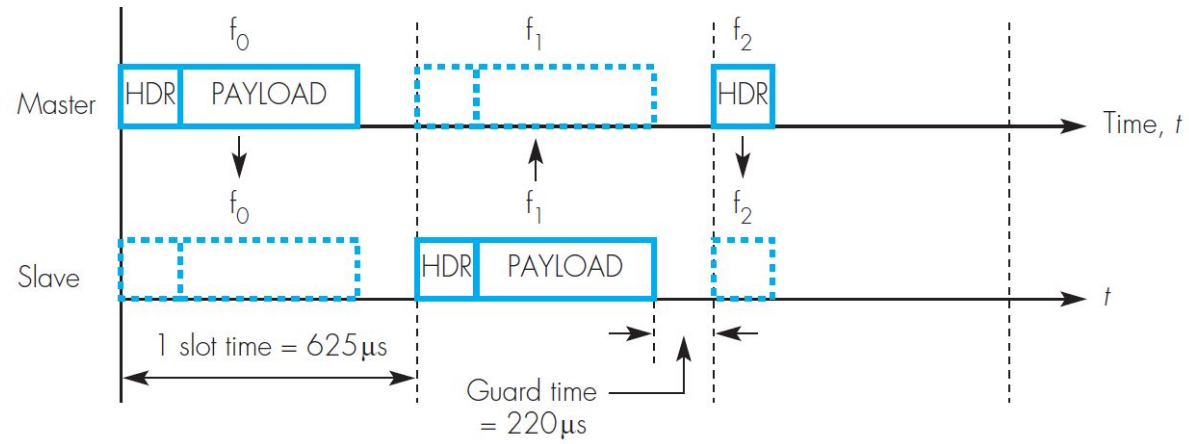
\includegraphics[width=0.9\linewidth]{img/wpan/picocomm}
\end{center}

%End L5